\section{Results and Empirical Diagnostics}
\label{sec:results}

\subsection{Cross-Axis Generalization Diagnostics}
\label{subsec:cross_axis}

To systematically interrogate the generalization capabilities and failure boundaries of molecular graph neural networks (GNNs) for refrigerant solubility prediction, we benchmarked the baseline pure-graph architecture ($M_0$) against the physics-regularized reduced thermodynamic coordinate model ($M_{\mathrm{reduced}}$) across five orthogonal out-of-distribution (OOD) test axes. Each axis probes an isolated distribution shift, spanning molecular identity (M1), matrix counter-ion class (B1, B2), compositional recombination (L2), and cross-chemical family saturation (HFO/HCFO zero-shot transfer). All performance statistics are frozen according to the authoritative project audit and reported in Table~\ref{tab:cross_axis_master} (5-seed mean metrics) and visualized in Figure~\ref{fig:figure1_ladder}.

\begin{table}[htbp]
\centering
\small
\caption{Cross-axis generalization benchmark comparing baseline pure-graph GNN ($M_0$) against reduced thermodynamic coordinate regularization ($M_{\mathrm{reduced}}$). Metrics represent the 5-seed mean for each axis. M1 is macro-averaged across 12 held-out HFC refrigerants; B1, B2, L2, and HFO/HCFO are pooled across test instances within each seed.}
\label{tab:cross_axis_master}
\begin{tabular}{llccccccc}
\toprule
\textbf{Axis} & \textbf{Distribution Shift Domain} & \textbf{$N_{\mathrm{test}}$} & \textbf{$M_0$ MAE} & \textbf{$M_{\mathrm{red}}$ MAE} & \textbf{$\Delta\text{MAE}$ (\%)} & \textbf{$M_0$ $R^2$} & \textbf{$M_{\mathrm{red}}$ $R^2$} & \textbf{$M_{\mathrm{red}}$ $\bar{\sigma}$} \\
\midrule
M1 & Refrigerant identity (12 HFC LORO) & 1403 & 0.1049 & 0.0666 & \textbf{−36.5\%} & −0.4158 & 0.3824 & — \\
B1 & High-redundancy anion (Fam-2 fluorosulfonates) & 513 & 0.0304 & 0.0302 & −0.7\% & 0.9265 & 0.9285 & 0.0092 \\
B2 & Inorganic fluoride anion (Fam-3 $\text{BF}_4/\text{PF}_6$) & 598 & 0.0534 & 0.0483 & −9.6\% & 0.7931 & 0.8333 & 0.0110 \\
L2 & Compositional recombination (4 unseen IL pairs) & 374 & 0.0334 & 0.0293 & −12.2\% & 0.8878 & 0.9126 & 0.0142 \\
HFO/HCFO & Unsaturated zero-shot cross-family transfer & 1106 & 0.0468 & 0.0326 & \textbf{−30.4\%} & 0.4920 & 0.6926 & 0.0144 \\
\bottomrule
\end{tabular}
\end{table}

\begin{figure}[htbp]
\centering
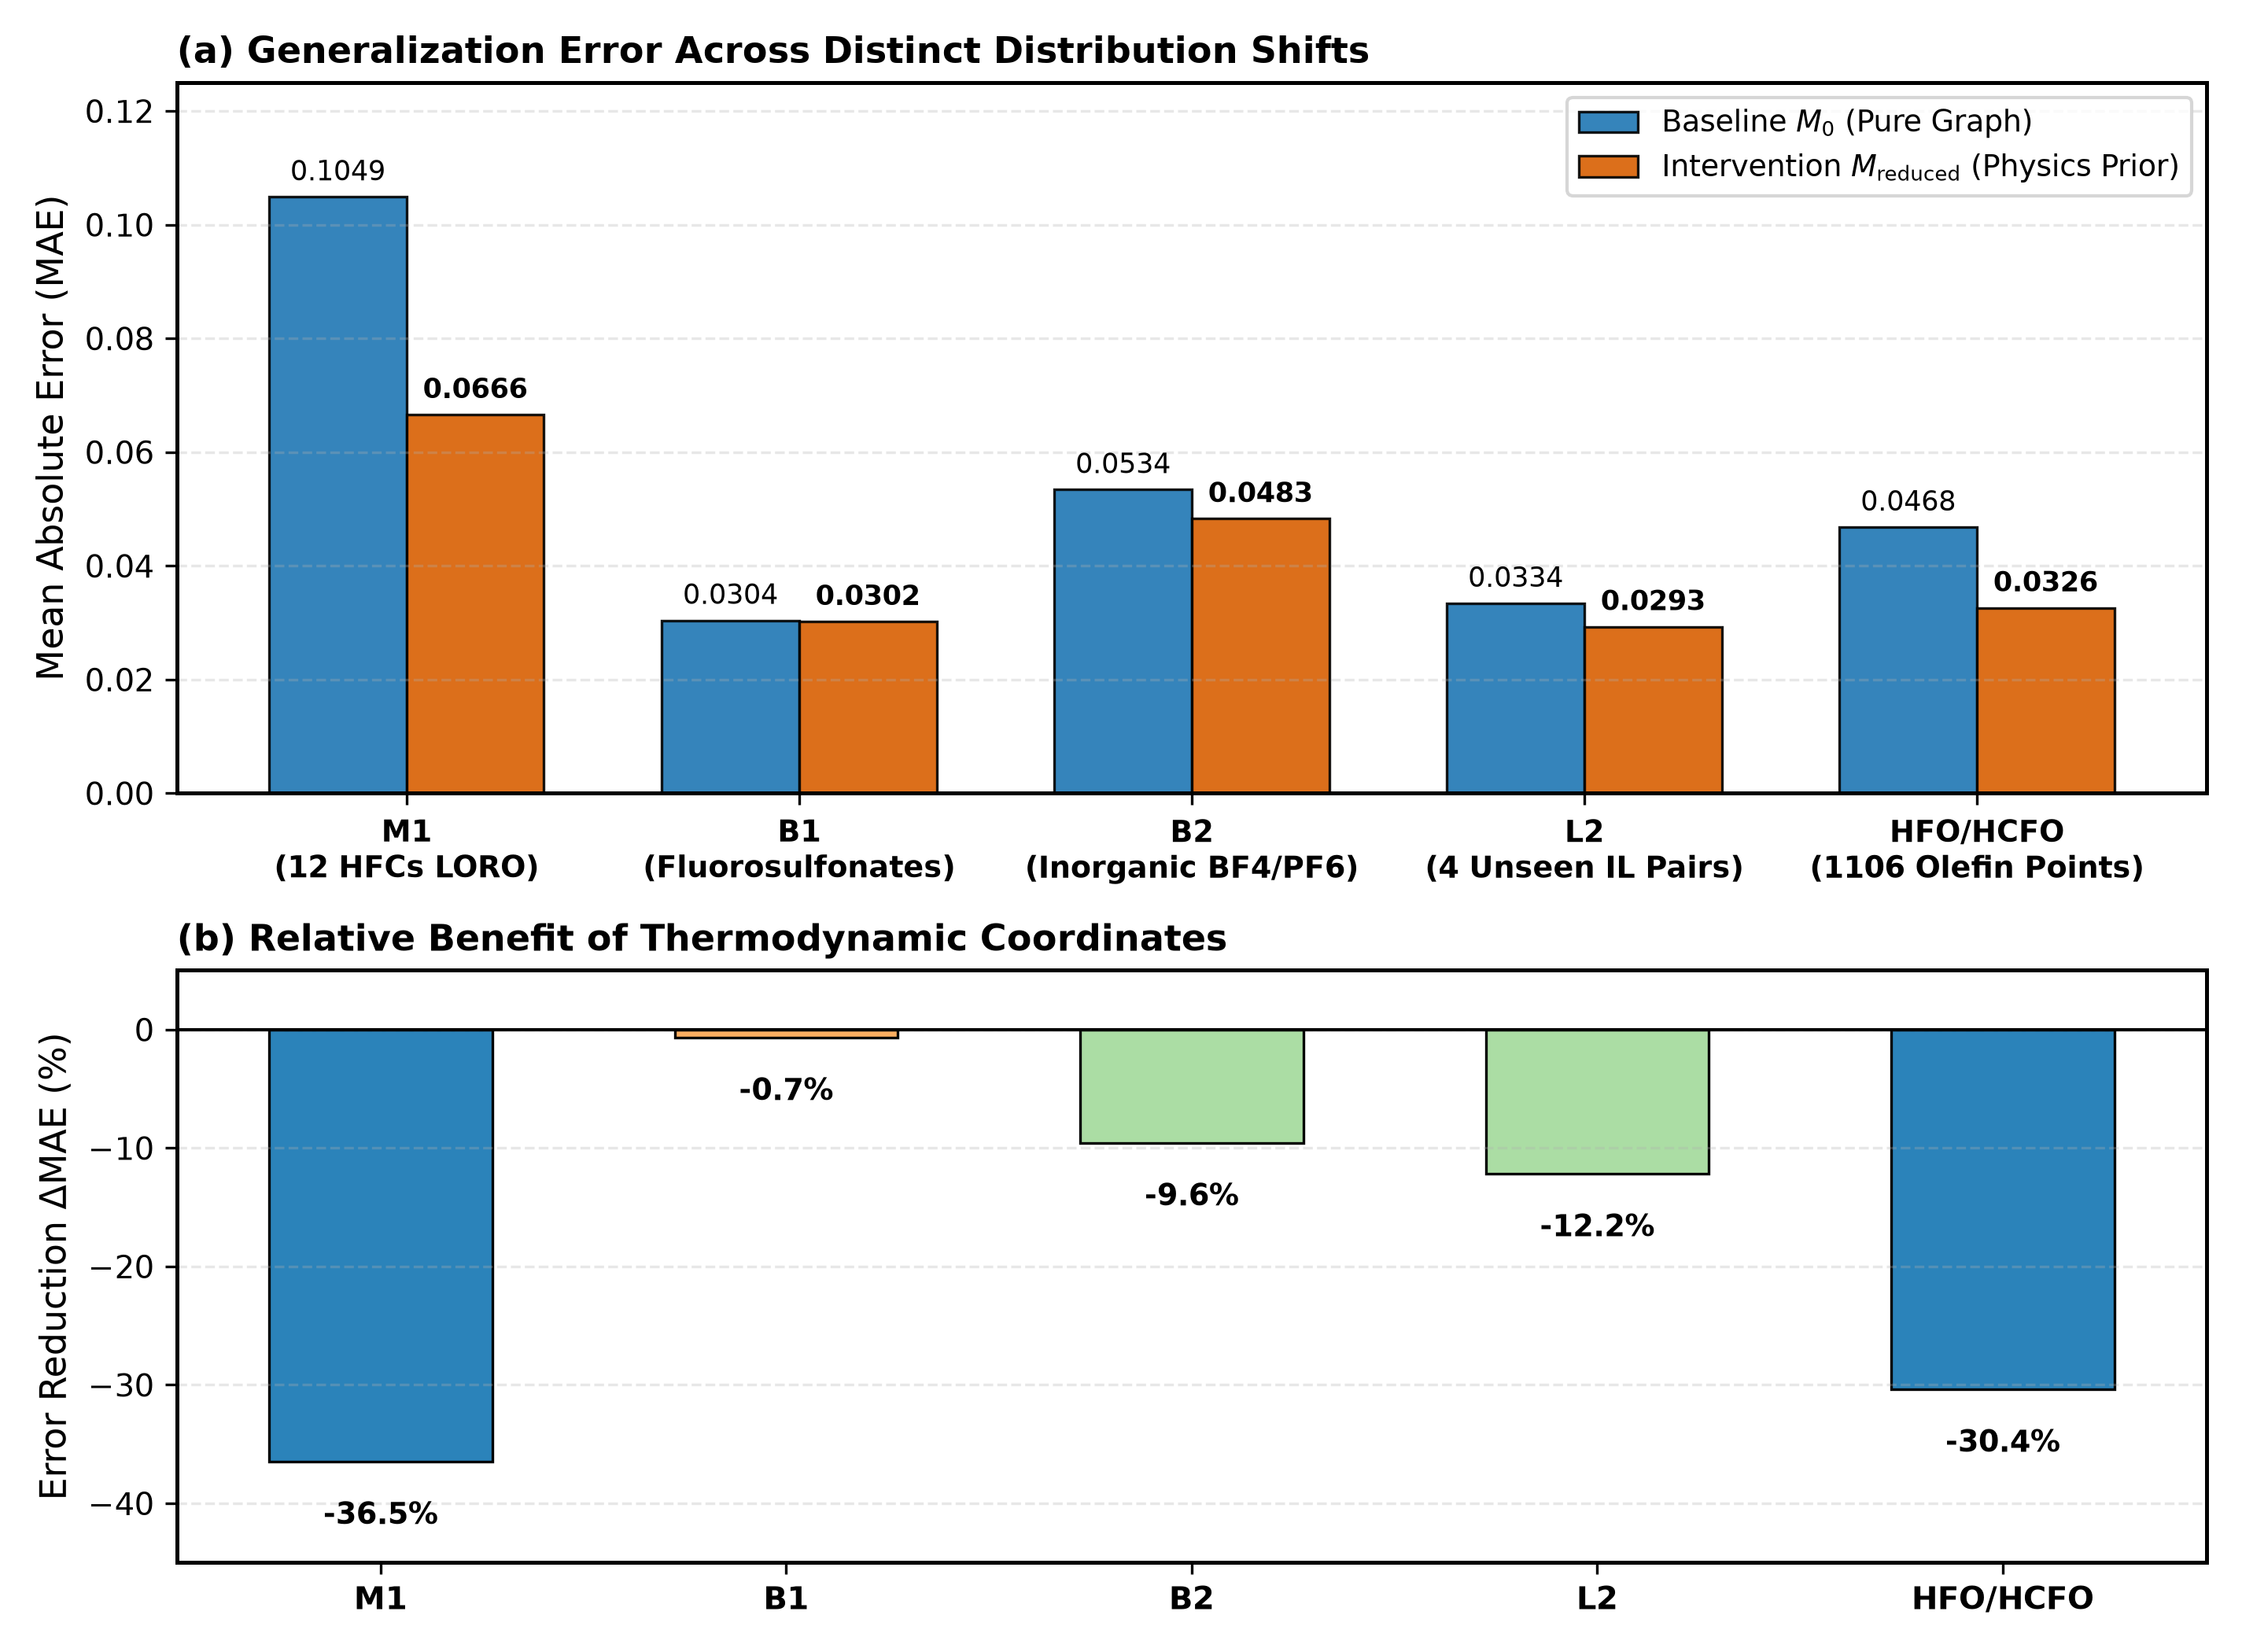
\includegraphics[width=0.85\linewidth]{figures/Figure1_chemical_generalization_ladder.pdf}
\caption{\textbf{Chemical generalization ladder across five orthogonal distribution shifts.} (a) Test mean absolute error (MAE) comparison between baseline pure-graph architecture ($M_0$, blue) and the reduced thermodynamic coordinate model ($M_{\mathrm{reduced}}$, orange). (b) Waterfall decomposition of relative error reduction $\Delta\text{MAE} = (\text{MAE}_{\mathrm{red}} - \text{MAE}_{0})/\text{MAE}_{0}$, demonstrating selective benefits in molecular extrapolation regimes (M1, HFO/HCFO) alongside limited impact in high-redundancy anion regimes (B1).}
\label{fig:figure1_ladder}
\end{figure}

As summarized in Table~\ref{tab:cross_axis_master} and Figure~\ref{fig:figure1_ladder}, distinct chemical shifts impose starkly disparate inductive challenges on the learned molecular representations:

\begin{enumerate}
    \item \textbf{Selective Benefit of Thermodynamic Coordinates}: Rather than yielding uniform error reductions across all benchmarks, the incorporation of corresponding-states thermodynamic coordinates ($T_r = T/T_c$, $P_r = P/P_c$, and Pitzer acentric factor $\omega$) selectively aids regimes where the molecular identity of the gas solute undergoes significant extrapolation. On the 12-refrigerant Leave-One-Refrigerant-Out (LORO, M1) benchmark ($N=1403$), baseline $M_0$ completely degenerates ($R^2 = -0.4158$, $\text{MAE} = 0.1049$), whereas $M_{\mathrm{reduced}}$ recovers positive predictive correlation ($R^2 = 0.3824$, $\text{MAE} = 0.0666$, a $-36.5\%$ error reduction). Similarly, under zero-shot transfer to unsaturated refrigerants ($N=1106$), $M_{\mathrm{reduced}}$ cuts test MAE from $0.0468$ to $0.0326$ ($-30.4\%$), elevating $R^2$ from $0.4920$ to $0.6926$.
    \item \textbf{Graph Redundancy Buffers Anion Shifts}: In contrast, when the shift is localized to the ionic liquid anion matrix where structural analogs are densely represented in the training set (e.g., Fam-2 fluorosulfonate anions, B1, $N=513$), baseline $M_0$ already maintains excellent fidelity ($\text{MAE} = 0.0304$, $R^2 = 0.9265$). Consequently, augmenting the scalar MLP branch with thermodynamic priors offers minimal marginal utility ($-0.7\%$ $\Delta\text{MAE}$, $\text{MAE} = 0.0302$).
    \item \textbf{Decoupled Coordination Geometries}: When shifting to compact inorganic anions ($\text{BF}_4^-$ and $\text{PF}_6^-$, B2, $N=598$), which feature symmetric coordination shells and substantially lower charge delocalization than bulky fluorosulfonates, baseline error increases to $0.0534$. Here, $M_{\mathrm{reduced}}$ provides moderate regularization, lowering MAE to $0.0483$ ($-9.6\%$, $R^2: 0.7931 \to 0.8333$).
\end{enumerate}

These comparative findings substantiate our central thesis: \textit{generalization difficulty cannot be abstracted as a monolithic property of deep molecular networks; rather, different chemical shifts trigger distinct representation bottlenecks, and macroscopic thermodynamic scaling coordinates regularize solute extrapolation while offering negligible impact when graph topological patterns are already redundant.}

\subsection{Compositional Generalization in Ionic Liquid Mixtures (L2 Benchmark)}
\label{subsec:l2_benchmark}

A prominent industrial advantage of ionic liquids is the synthetic versatility of cation--anion pairing. However, evaluating whether GNNs truly learn compositional interactions or merely memorize individual component marginals requires testing on entirely unseen cation--anion recombinations where both the cation and the anion have appeared in the training corpus, but never in mutual combination.

The L2 benchmark rigorously enforces this protocol across $N=374$ test instances distributed over four distinct ionic pairs: $[\text{emim}][\text{BF}_4]$ ($N=93$), $[\text{emim}][\text{OTf}]$ ($N=114$), $[\text{bmim}][\text{OTf}]$ ($N=50$), and $[\text{hmim}][\text{BF}_4]$ ($N=117$). In addition to the 5-seed pooled performance reported in Table~\ref{tab:cross_axis_master} ($M_0$ MAE $0.0334 \to M_{\mathrm{reduced}}$ MAE $0.0293$, $-12.2\%$), we conducted an ensemble prediction analysis and fine-grained pair-level paired effect test, presented in Table~\ref{tab:l2_pairs}.

\begin{table}[htbp]
\centering
\small
\caption{Pair-level compositional generalization performance on the L2 benchmark ($N=374$). Metrics reflect 5-seed ensemble predictions.}
\label{tab:l2_pairs}
\begin{tabular}{lcccccc}
\toprule
\textbf{Held-out Ionic Pair} & \textbf{$N$} & \textbf{$M_0$ Ensemble MAE} & \textbf{$M_{\mathrm{red}}$ Ensemble MAE} & \textbf{$\Delta\text{MAE}$ (\%)} & \textbf{$M_{\mathrm{red}}$ $R^2$} & \textbf{$M_{\mathrm{red}}$ $\bar{\sigma}$} \\
\midrule
$[\text{emim}][\text{BF}_4]$ & 93 & 0.0264 & 0.0207 & \textbf{−21.6\%} & 0.9652 & 0.0153 \\
$[\text{emim}][\text{OTf}]$ & 114 & 0.0294 & 0.0274 & −6.7\% & 0.8838 & 0.0129 \\
$[\text{bmim}][\text{OTf}]$ & 50 & 0.0437 & 0.0407 & −7.0\% & 0.8768 & 0.0121 \\
$[\text{hmim}][\text{BF}_4]$ & 117 & 0.0270 & 0.0260 & −3.5\% & 0.8960 & 0.0157 \\
\midrule
\textbf{Pooled L2 Ensemble} & \textbf{374} & \textbf{0.0298} & \textbf{0.0271} & \textbf{−9.1\%} & \textbf{0.9218} & \textbf{0.0142} \\
\bottomrule
\end{tabular}
\end{table}

To confirm that the observed error reduction is not an artifact of random seed selection or driven by outliers in a single system, we executed a rigorous point-wise paired statistical test over all 374 points ($e_i^{(0)} = |y_i - \hat{y}_i^{(M_0)}|$, $e_i^{(\mathrm{red})} = |y_i - \hat{y}_i^{(M_{\mathrm{red}})}|$):
\begin{itemize}
    \item \textbf{Mean Paired Effect}: $\Delta e = e^{(0)} - e^{(\mathrm{red})} = 0.002724$.
    \item \textbf{Bootstrap 95\% Confidence Interval}: Resampling 10,000 bootstrap replicates yielded a 95\% confidence interval of $[0.001515, 0.003915]$, cleanly excluding zero and confirming statistical significance at $\alpha = 0.05$.
    \item \textbf{Non-Parametric Hypothesis Testing}: A one-sided Wilcoxon signed-rank test confirmed that $M_{\mathrm{reduced}}$ absolute errors are systematically smaller than $M_0$ ($W = 44102.0$, $p = 5.18 \times 10^{-6}$).
    \item \textbf{Pairwise Win Rate}: Across all 374 points, $M_{\mathrm{reduced}}$ achieved lower absolute error in $59.9\%$ of test instances.
\end{itemize}

Pair-level inspection (Table~\ref{tab:l2_pairs}) demonstrates that error reduction is most pronounced in $[\text{emim}][\text{BF}_4]$ ($\text{MAE}: 0.0264 \to 0.0207$, $-21.6\%$, $R^2 = 0.9652$), an ionic liquid whose constituent $[\text{emim}]^+$ and $[\text{BF}_4]^-$ ions possess strong electrostatic charge density and pronounced temperature-dependent packing behaviors that are effectively normalized by critical coordinate scaling.

\subsection{Continuous Generalization Landscape and Chemical Distance}
\label{subsec:continuous_landscape}

A widespread premise in molecular machine learning is that OOD generalization error correlates monotonically with the chemical distance between the test query and the training distribution. Under this hypothesis, failure boundaries could be anticipated simply by computing a distance threshold. To examine whether this premise holds in multicomponent absorption thermodynamics, we mapped the point-wise and species-level test errors against three continuous distance metrics (Figure~\ref{fig:figure2_landscape}):
\begin{enumerate}
    \item \textbf{Topological Distance ($D_{\mathrm{FP}}$)}: $1 - \text{Tanimoto similarity}$ evaluated on 2048-bit Morgan circular fingerprints (radius 2).
    \item \textbf{Physicochemical Distance ($D_{\mathrm{phys}}$)}: Normalized Euclidean distance over computed RDKit molecular descriptors (molecular weight, partial charge extremes, $\text{MolLogP}$, TPSA).
    \item \textbf{Critical Thermodynamic Distance ($D_{\mathrm{thermo}}$)}: Normalized Euclidean distance in the critical parameter manifold ($T_c, P_c, \omega$).
\end{enumerate}

\begin{figure}[htbp]
\centering
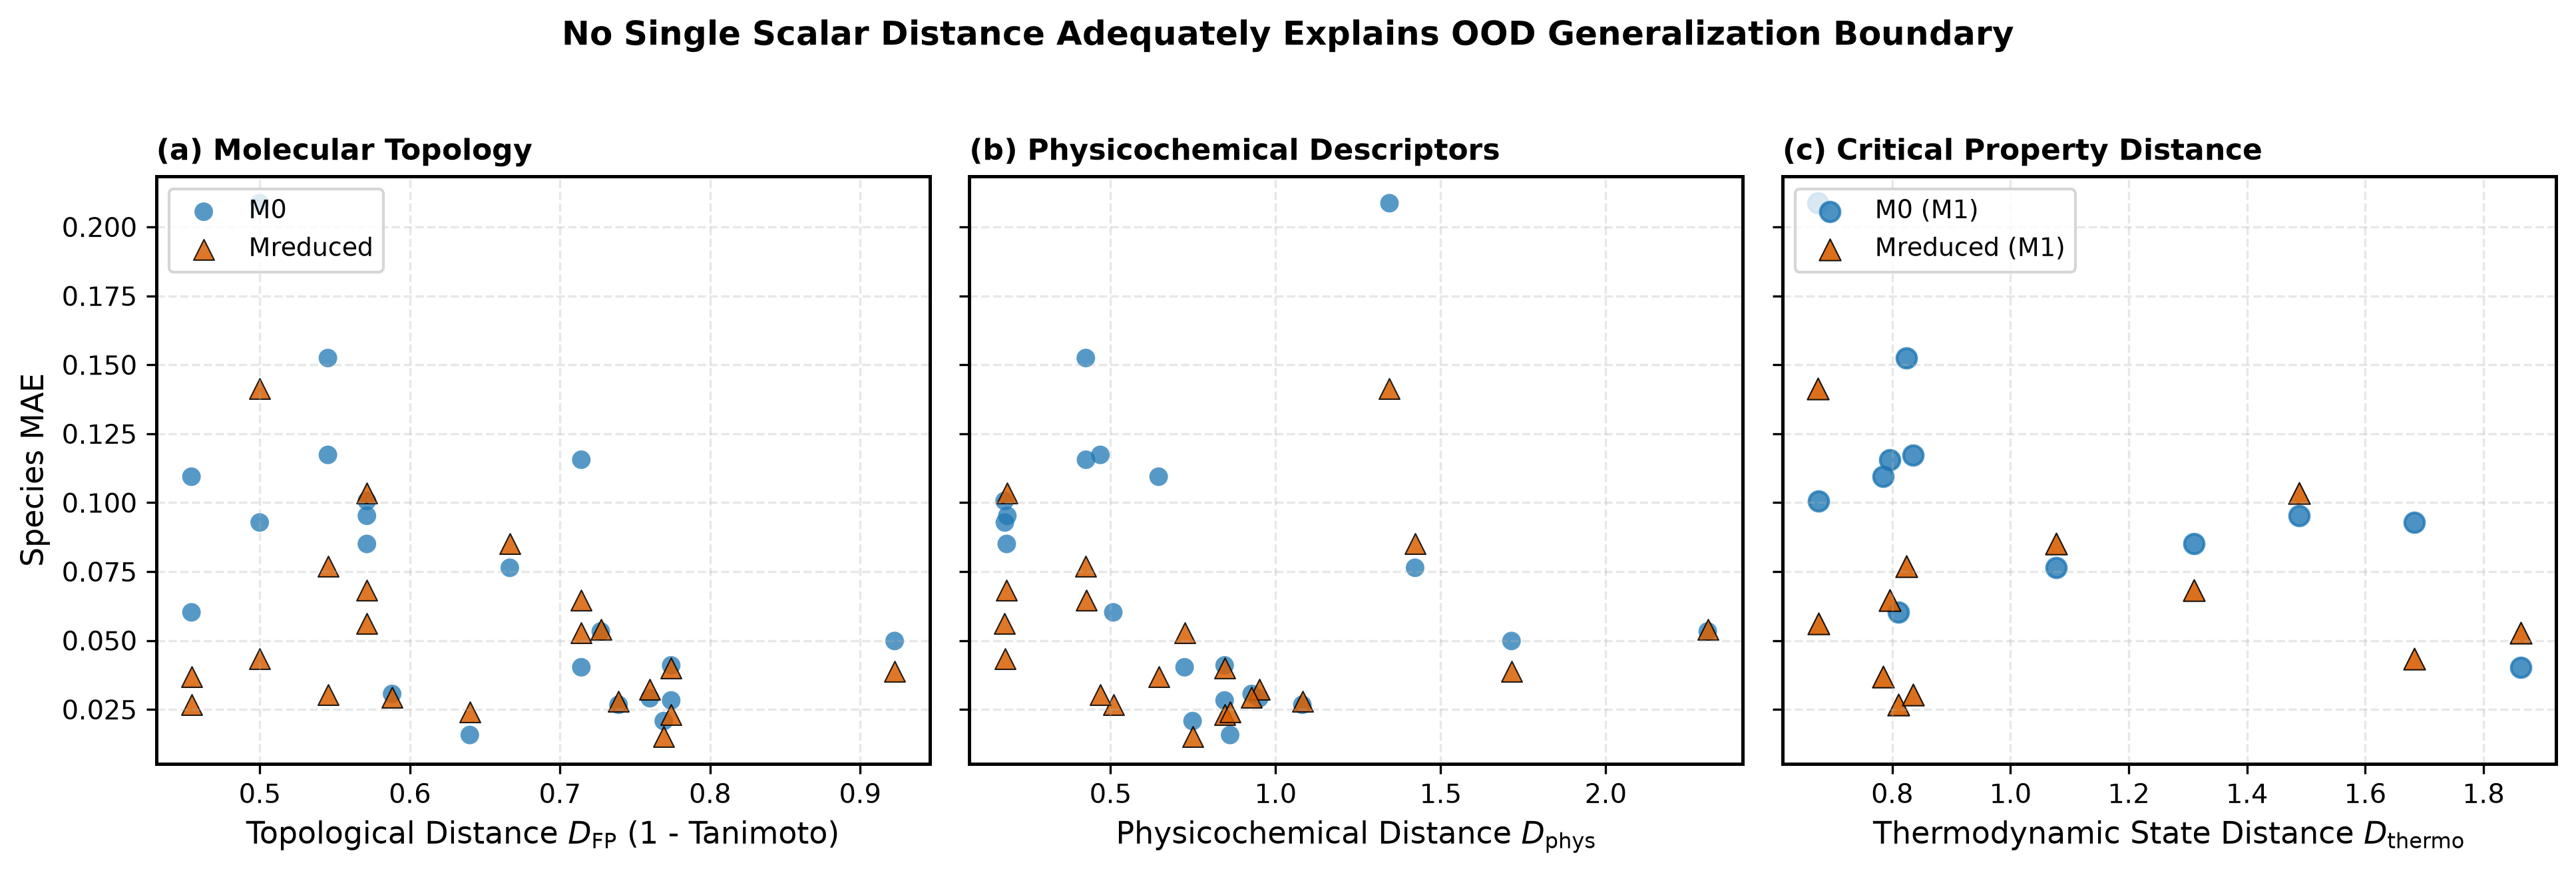
\includegraphics[width=\linewidth]{figures/Figure2_continuous_generalization_landscape.pdf}
\caption{\textbf{Continuous generalization landscape across topological, physicochemical, and thermodynamic dimensions.} (a) Species-level MAE versus Morgan fingerprint topological distance $D_{\mathrm{FP}}$. (b) Species-level MAE versus physicochemical descriptor distance $D_{\mathrm{phys}}$. (c) Species-level MAE versus critical property distance $D_{\mathrm{thermo}}$ for the M1 LORO benchmark. Across all three projections, error does not scale monotonically with scalar distance, refuting simple threshold models of OOD generalization.}
\label{fig:figure2_landscape}
\end{figure}

As revealed in Figure~\ref{fig:figure2_landscape}, empirical test errors scatter broadly across all three metrics, and \textbf{no single scalar distance adequately explains the observed generalization boundary}:
\begin{itemize}
    \item In the topological projection (Figure~\ref{fig:figure2_landscape}a), solutes with moderate distance to the nearest training solute ($D_{\mathrm{FP}}^{\mathrm{NN-train}} \approx 0.55$) exhibit higher test MAE ($>0.15$ in $M_0$) than solutes located at severe topological distances ($D_{\mathrm{FP}}^{\mathrm{NN-train}} > 0.90$, $\text{MAE} \approx 0.05$). Furthermore, while the inter-isomer structural distance between R134 and R134a is substantial ($D_{\mathrm{FP}}^{\mathrm{pair}} \approx 0.9167$, $D_{\mathrm{phys}}^{\mathrm{pair}} \approx 0.0833$), both isomers reside at virtually identical distance to the nearest training solute ($D_{\mathrm{FP}}^{\mathrm{NN-train}} \approx 0.50\text{--}0.55$, $D_{\mathrm{phys}}^{\mathrm{NN-train}} \approx 0.0805\text{--}0.0807$).
    \item In the physicochemical space (Figure~\ref{fig:figure2_landscape}b), despite identical formulas ($\text{C}_2\text{H}_2\text{F}_4$) and nearly indistinguishable $D_{\mathrm{phys}}^{\mathrm{NN-train}}$, baseline $M_0$ exhibits pronounced extrapolation divergence ($\text{MAE} = 0.2086$ for R134 vs $0.1525$ for R134a), which persists under thermodynamic grounding ($M_{\mathrm{reduced}}\text{ MAE}: 0.1414$ vs $0.0769$).
    \item In the thermodynamic projection (Figure~\ref{fig:figure2_landscape}c), while $D_{\mathrm{thermo}}$ correlates somewhat better with failure in M1 LORO, points with $D_{\mathrm{thermo}} > 1.6$ (e.g., R227ea) can achieve lower prediction errors ($\text{MAE} \approx 0.04$) than points with $D_{\mathrm{thermo}} \approx 0.8$ (e.g., R143a, $\text{MAE} > 0.11$).
\end{itemize}

Consequently, failure in molecular GNNs is not dictated by smooth distance metrics along arbitrary 1D manifolds. Rather, failure arises from \textbf{discrete representational blind spots}---such as internal charge dipole cancellation, stereoisomerism, or altered local coordination geometry---which cannot be captured by global scalar similarity metrics.

\subsection{Zero-Shot Cross-Family Transfer to Unsaturated Refrigerants}
\label{subsec:unsat_transfer}

To evaluate whether representations trained exclusively on saturated hydrofluorocarbons (HFCs, 2739 points) can transfer to fourth-generation low-global-warming-potential (GWP) fluorinated olefins, we probed the All-HFC model on an external benchmark of $N=1106$ unsaturated points spanning hydrofluoroolefins (HFOs) and hydrochlorofluoroolefins (HCFOs). The species-level results are summarized in Table~\ref{tab:unsat_species}.

\begin{table}[htbp]
\centering
\small
\caption{Species-level zero-shot transfer performance to unsaturated refrigerants under the All-HFC training protocol ($N_{\mathrm{test}}=1106$). Models were trained without any olefinic samples.}
\label{tab:unsat_species}
\begin{tabular}{llccccccc}
\toprule
\textbf{Species} & \textbf{Class} & \textbf{$N$} & \textbf{$M_0$ MAE} & \textbf{$M_{\mathrm{red}}$ MAE} & \textbf{$\Delta\text{MAE}$ (\%)} & \textbf{$M_0$ $R^2$} & \textbf{$M_{\mathrm{red}}$ $R^2$} & \textbf{$M_{\mathrm{red}}$ $\bar{\sigma}$} \\
\midrule
R1234yf & HFO (propene) & 685 & 0.0320 & 0.0250 & \textbf{−21.9\%} & 0.7240 & 0.8017 & 0.0134 \\
R1234ze(E) & HFO (propene) & 308 & 0.0391 & 0.0303 & \textbf{−22.5\%} & 0.5433 & 0.7614 & 0.0158 \\
R1233zd(E) & HCFO (chloro-olefin) & 90 & 0.0297 & 0.0193 & \textbf{−35.2\%} & −0.4074 & 0.2307 & 0.0165 \\
R1336mzz(E) & HFO (butene, trans) & 11 & 0.1196 & 0.2885 & +141.1\% & −9.0666 & −53.4281 & 0.0213 \\
R1336mzz(Z) & HFO (butene, cis) & 12 & 0.2854 & 0.1536 & \textbf{−46.2\%} & −3.3085 & −0.6739 & 0.0116 \\
\midrule
\textbf{Total Unsaturated} & \textbf{Pooled} & \textbf{1106} & \textbf{0.0374} & \textbf{0.0300} & \textbf{−19.8\%} & \textbf{0.6227} & \textbf{0.7107} & \textbf{0.0144} \\
\bottomrule
\end{tabular}
\end{table}

\subsubsection{Robust Cross-Family Generalization in Mainstream Olefins}
For the predominant commercial refrigerants R1234yf ($N=685$) and R1234ze(E) ($N=308$), zero-shot transfer is remarkably robust:
\begin{itemize}
    \item For R1234yf, $M_{\mathrm{reduced}}$ achieves an ensemble MAE of $0.0250$ ($R^2 = 0.8017$), outperforming baseline $M_0$ ($0.0320$, $R^2 = 0.7240$) by $21.9\%$.
    \item For R1234ze(E), MAE drops from $0.0391$ to $0.0303$ ($-22.5\%$), with $R^2$ advancing from $0.5433$ to $0.7614$.
    \item For the chloro-fluoroolefin R1233zd(E) ($N=90$), despite the model never encountering a chlorine atom bonded to an unsaturated framework in training, $M_{\mathrm{reduced}}$ reduces MAE to $0.0193$ ($-35.2\%$).
\end{itemize}

To ensure that this overall performance gain is not solely an artifact of R1233zd(E), a sensitivity audit on the pure-HFO subset ($N=1016$, excluding R1233zd(E)) confirms an identical pattern: MAE drops from $0.0381 \to 0.0310$ ($-18.7\%$, $R^2: 0.622 \to 0.708$).

\subsubsection{Failure Boundary: Stereochemical Degeneracy in R1336mzz Isomers}
In sharp contrast to the fluoropropenes, the hexafluorobutene isomers R1336mzz(E) and R1336mzz(Z) expose an acute failure boundary (Table~\ref{tab:unsat_species} and Figure~\ref{fig:figure5_boundary}):
\begin{itemize}
    \item Under baseline $M_0$, both isomers exhibit severe degradation, with MAEs exceeding $0.11$ and $0.28$, respectively, and negative $R^2$ scores.
    \item Under $M_{\mathrm{reduced}}$, the cis-isomer R1336mzz(Z) improves substantially ($\text{MAE}: 0.2854 \to 0.1536$, a $46.2\%$ reduction), whereas the trans-isomer R1336mzz(E) undergoes severe negative transfer ($\text{MAE}: 0.1196 \to 0.2885$, $+141.1\%$).
\end{itemize}

This divergent behavior stems from a fundamental representational limitation: in standard 2D molecular graph featurization, graph connectivity and atom node features do not explicitly encode double-bond cis/trans stereochemical configurations. Consequently, the message passing branches produce mathematically degenerate representations ($G_E \equiv G_Z$). When $M_{\mathrm{reduced}}$ introduces species-dependent critical coordinates ($T_c, P_c, \omega$), the model distinguishes the two molecules through the scalar MLP branch; however, because the underlying graph embedding is uninformative regarding spatial configuration, the shift in scalar conditioning is associated with opposite changes in the two isomers, improving R1336mzz(Z) while substantially degrading R1336mzz(E).

\subsection{Mechanistic Attribution and Physical Prior Grounding}
\label{subsec:mechanistic_attribution}

To elucidate \textit{why} reduced thermodynamic coordinates improve generalization in some regimes while remaining passive in others, we performed feature attribution via Integrated Gradients (IG) across the model's multi-branch architecture. Attributions were aggregated into five chemically coherent concept groups:
\begin{enumerate}
    \item \textbf{Thermodynamic State}: Ambient operating conditions ($T, P$).
    \item \textbf{Refrigerant Physicochemical Features}: Molecular descriptors of the solute ($q_{\mathrm{max}}, \text{MolLogP}, \text{MW}$).
    \item \textbf{Anion Descriptors}: Molecular weight and charge attributes of the anion.
    \item \textbf{Cation Descriptors}: Polar surface area, charge extremes, and weight of the cation.
    \item \textbf{Reduced Thermodynamic Coordinates}: Dimensionless scaling priors ($T_r, P_r, \omega$).
\end{enumerate}

Figure~\ref{fig:figure3_attribution} illustrates the redistribution of attribution shares between baseline $M_0$ and $M_{\mathrm{reduced}}$ for representative ionic liquid systems based on $\text{BF}_4^-$ and $\text{PF}_6^-$ anions.

\begin{figure}[htbp]
\centering
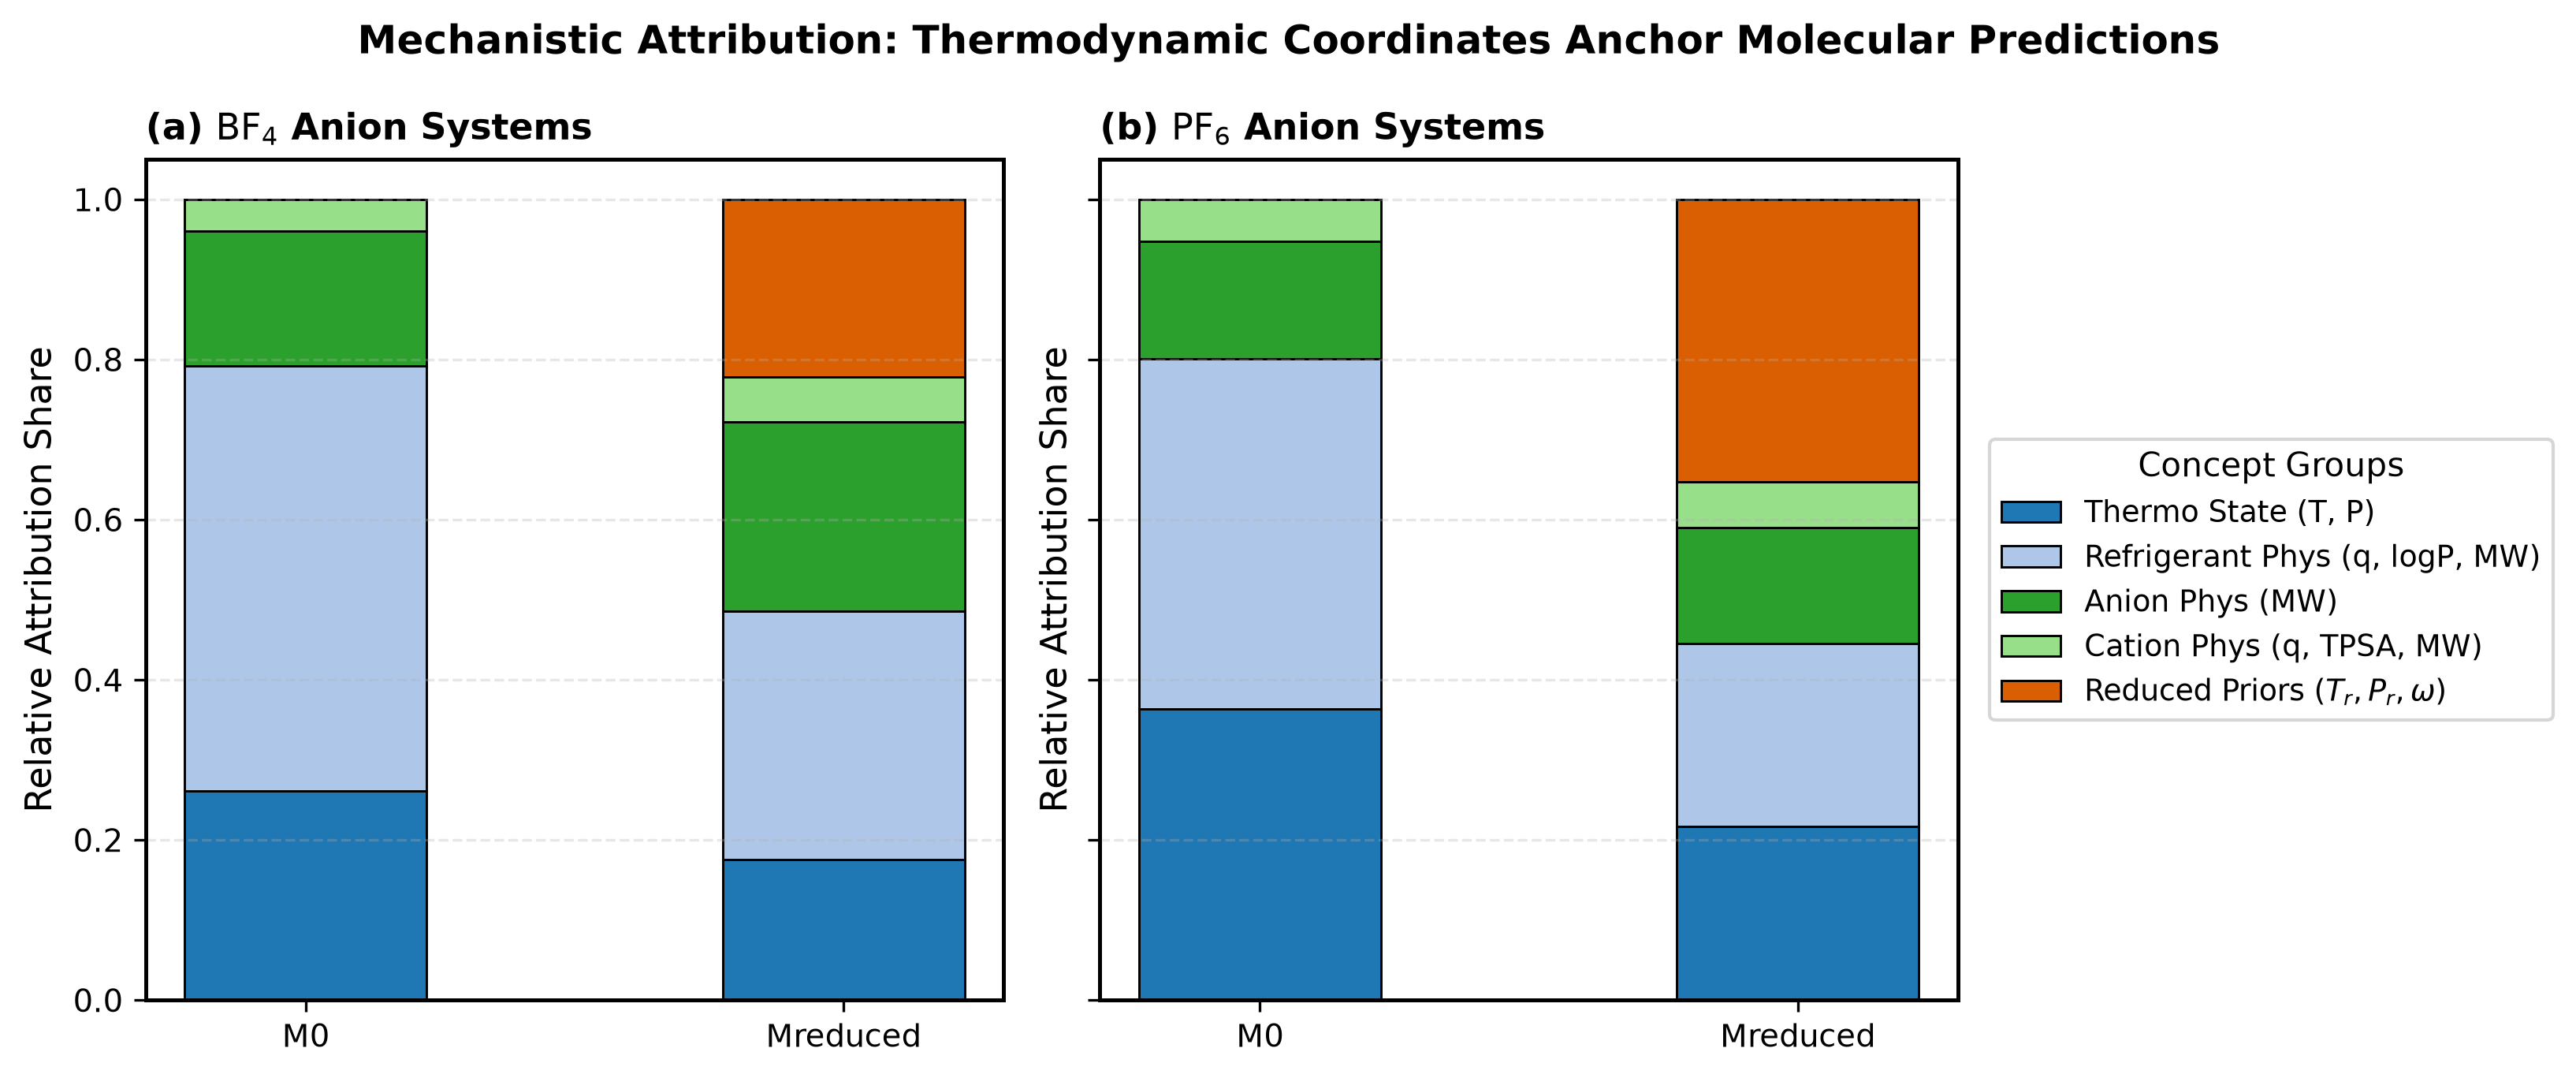
\includegraphics[width=0.88\linewidth]{figures/Figure3_mechanistic_attribution_ig.pdf}
\caption{\textbf{Mechanistic feature attribution via Integrated Gradients.} Relative concept share redistribution between baseline $M_0$ and intervention $M_{\mathrm{reduced}}$ across (a) $\text{BF}_4^-$ and (b) $\text{PF}_6^-$ ionic liquid systems. Thermodynamic coordinates ($T_r, P_r, \omega$, orange) absorb over $22\%\sim35\%$ of total attribution weight, directly displacing unregularized refrigerant scalar descriptors (light blue) while stabilizing ambient state and ionic matrix contributions.}
\label{fig:figure3_attribution}
\end{figure}

In the baseline $M_0$ model, the decision process is heavily dominated by ambient state variables ($T, P$, accounting for $26\%\sim36\%$ of total attribution) and refrigerant scalar descriptors ($\sim43\%\sim53\%$), leaving the graph-derived ionic embeddings vulnerable to spurious shortcuts. When $M_{\mathrm{reduced}}$ is introduced, the reduced priors ($T_r, P_r, \omega$) absorb a substantial attribution fraction ($22.3\%$ in $\text{BF}_4$ and $35.4\%$ in $\text{PF}_6$). Crucially, this absorption primarily displaces the unregularized refrigerant descriptor share (which contracts from $53.0\%$ to $30.8\%$ in $\text{BF}_4$, and from $43.8\%$ to $22.6\%$ in $\text{PF}_6$), while preserving the structural attribution of the ionic liquid cation and anion. 

This mechanistic rebalancing is consistent with an \textbf{anchoring inductive bias}: by explicitly supplying corresponding-states coordinates, the model's reliance shifts toward dimensionless thermodynamic scaling rather than fitting fragile, dataset-dependent correlations between raw molecular descriptors and solubility values.

\subsection{Epistemic Uncertainty and Selective Decision-Making}
\label{subsec:uncertainty_risk}

For safety-critical chemical process design, an OOD-aware model must not only generate point predictions but also accurately signal when its predictions are untrustworthy. We quantified epistemic uncertainty using the seed-ensemble disagreement $\sigma_i = \mathrm{std}(\{\hat{y}_i^{(s)}\}_{s=1}^5)$ across the five independently trained seeds. The uncertainty landscape and risk-coverage decision curves are detailed in Table~\ref{tab:uncertainty_risk} and Figure~\ref{fig:figure4_uq}.

\begin{table}[htbp]
\centering
\small
\caption{Ensemble epistemic uncertainty diagnostics and selective prediction risk reduction across all five OOD benchmark axes under the $M_{\mathrm{reduced}}$ model. Note that for M1, the reported ensemble MAE is macro-averaged across the 12 held-out refrigerants to weight each chemical species equally, whereas risk--coverage values evaluate pooled test points directly.}
\label{tab:uncertainty_risk}
\begin{tabular}{lccccccp{3.5cm}}
\toprule
\textbf{Axis} & \textbf{$N_{\mathrm{test}}$} & \textbf{Ensemble MAE} & \textbf{Mean Disagreement $\bar{\sigma}$} & \textbf{Spearman $\rho(\sigma, |e|)$} & \textbf{Risk at 100\%} & \textbf{Risk at 50\% (MAE)} & \textbf{Aggregation Basis} \\
\midrule
M1 (LORO) & 1403 & 0.0613 & — & 0.3058 & 0.0720 & \textbf{0.0524 (−27.2\%)} & Macro across 12 refrigerants (MAE); pooled points (Risk) \\
B1 (Fam-2) & 513 & 0.0292 & 0.0092 & 0.5062 & 0.0292 & \textbf{0.0139 (−52.5\%)} & Pooled test points \\
B2 (Fam-3) & 598 & 0.0476 & 0.0110 & 0.6101 & 0.0472 & \textbf{0.0230 (−51.2\%)} & Pooled test points \\
L2 (Unseen Pairs) & 374 & 0.0271 & 0.0142 & 0.3084 & 0.0271 & \textbf{0.0201 (−25.8\%)} & Pooled test points \\
HFO/HCFO & 1106 & 0.0300 & 0.0144 & 0.4926 & 0.0300 & \textbf{0.0197 (−34.4\%)} & Pooled test points \\
\bottomrule
\end{tabular}
\end{table}

\begin{figure}[htbp]
\centering
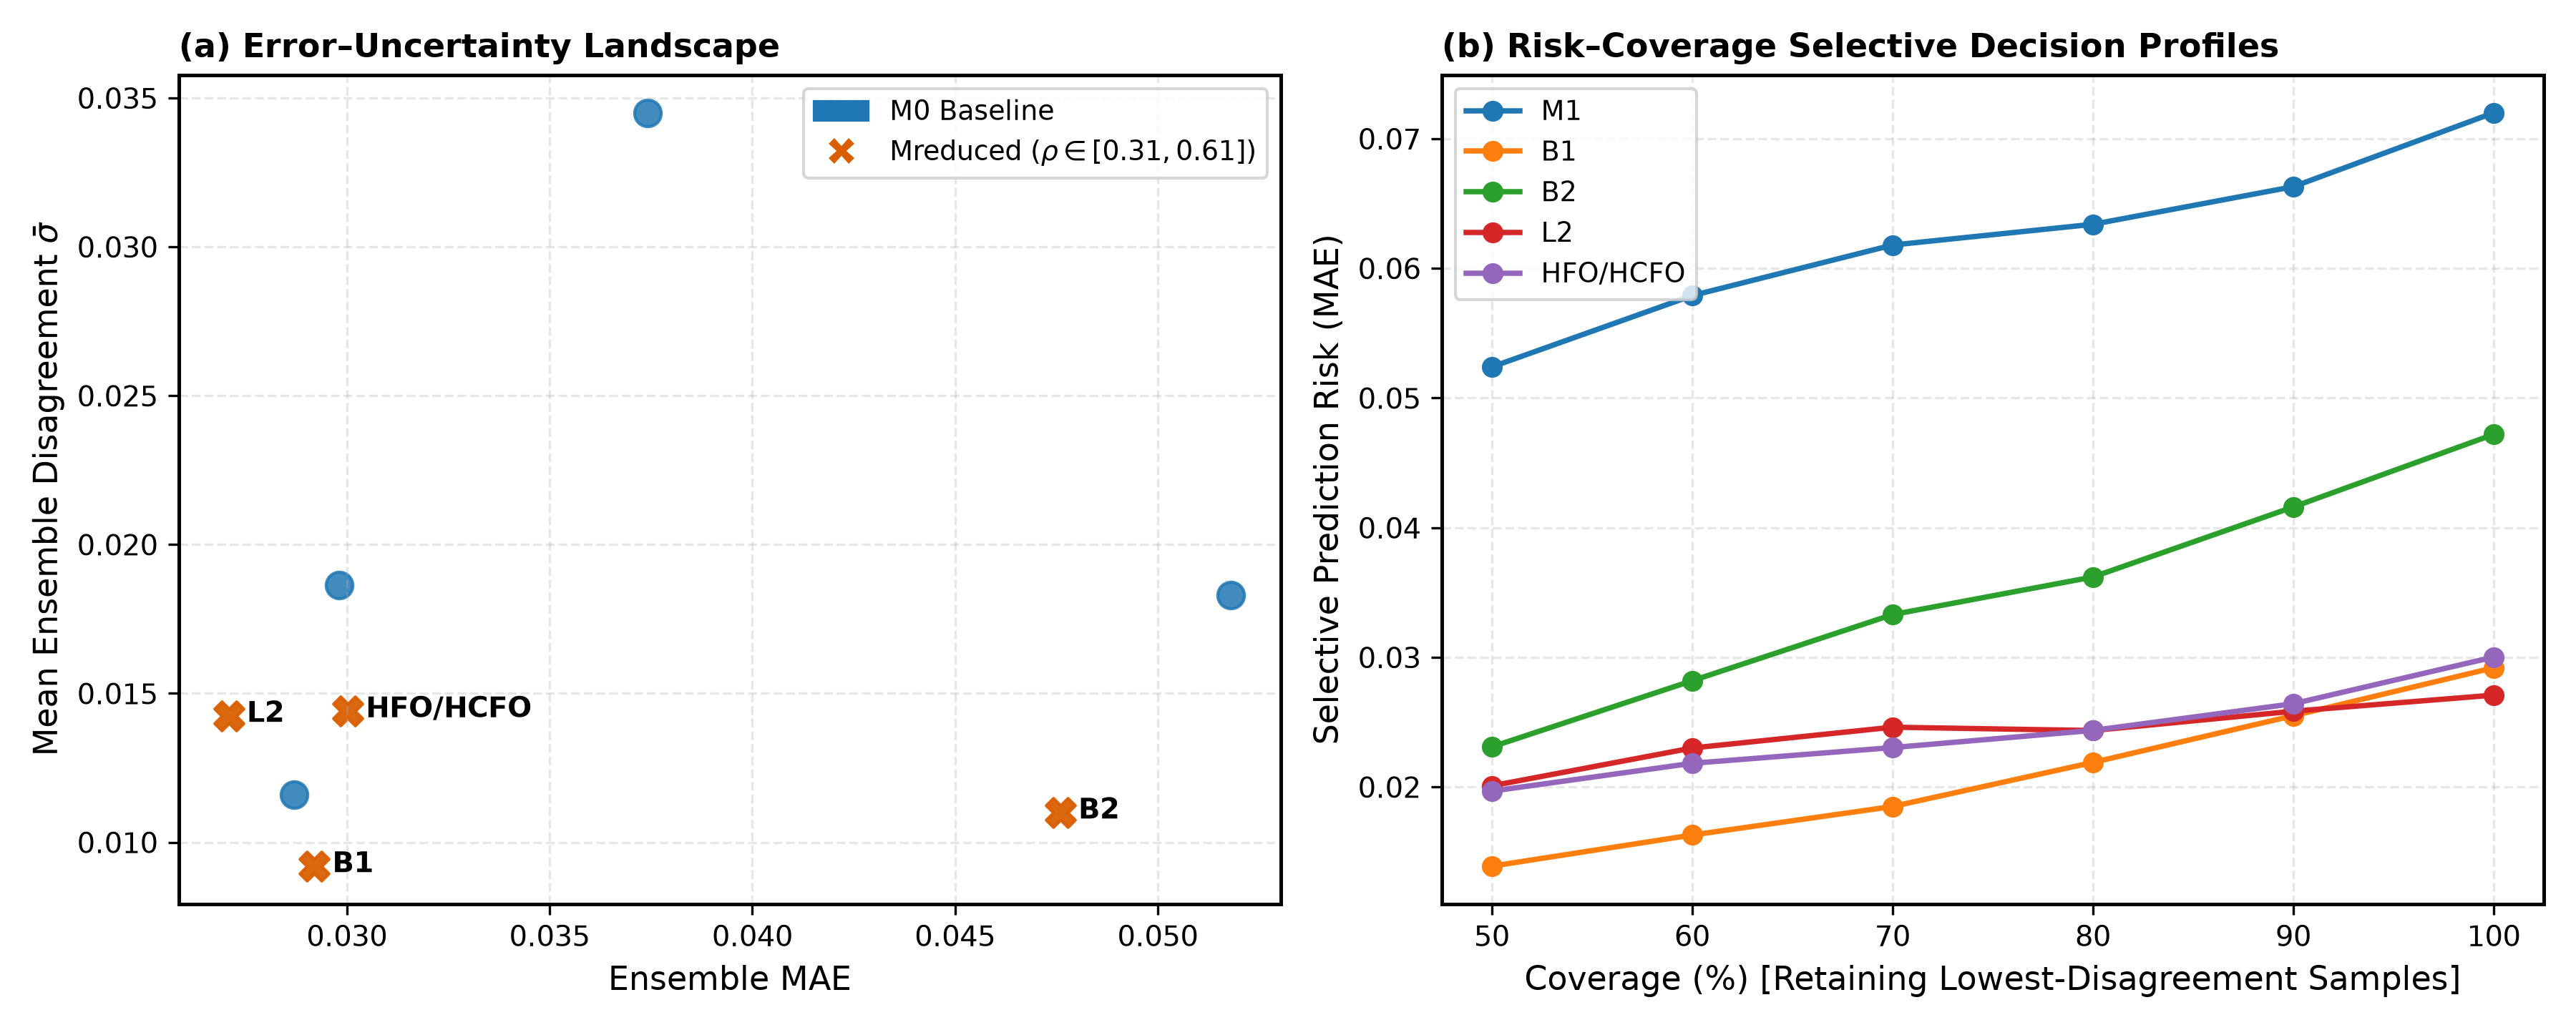
\includegraphics[width=\linewidth]{figures/Figure4_uncertainty_and_risk_coverage.pdf}
\caption{\textbf{Epistemic uncertainty reliability and selective prediction risk--coverage profiles.} (a) Error--uncertainty landscape plotting ensemble MAE against mean seed-ensemble disagreement $\bar{\sigma}$ across OOD benchmarks. (b) Risk--coverage curves under $M_{\mathrm{reduced}}$, where test points with the highest ensemble disagreement are progressively rejected. Retaining the 50\% highest-confidence predictions cuts risk by $25.8\%\sim52.5\%$ across all axes.}
\label{fig:figure4_uq}
\end{figure}

\begin{figure}[htbp]
\centering
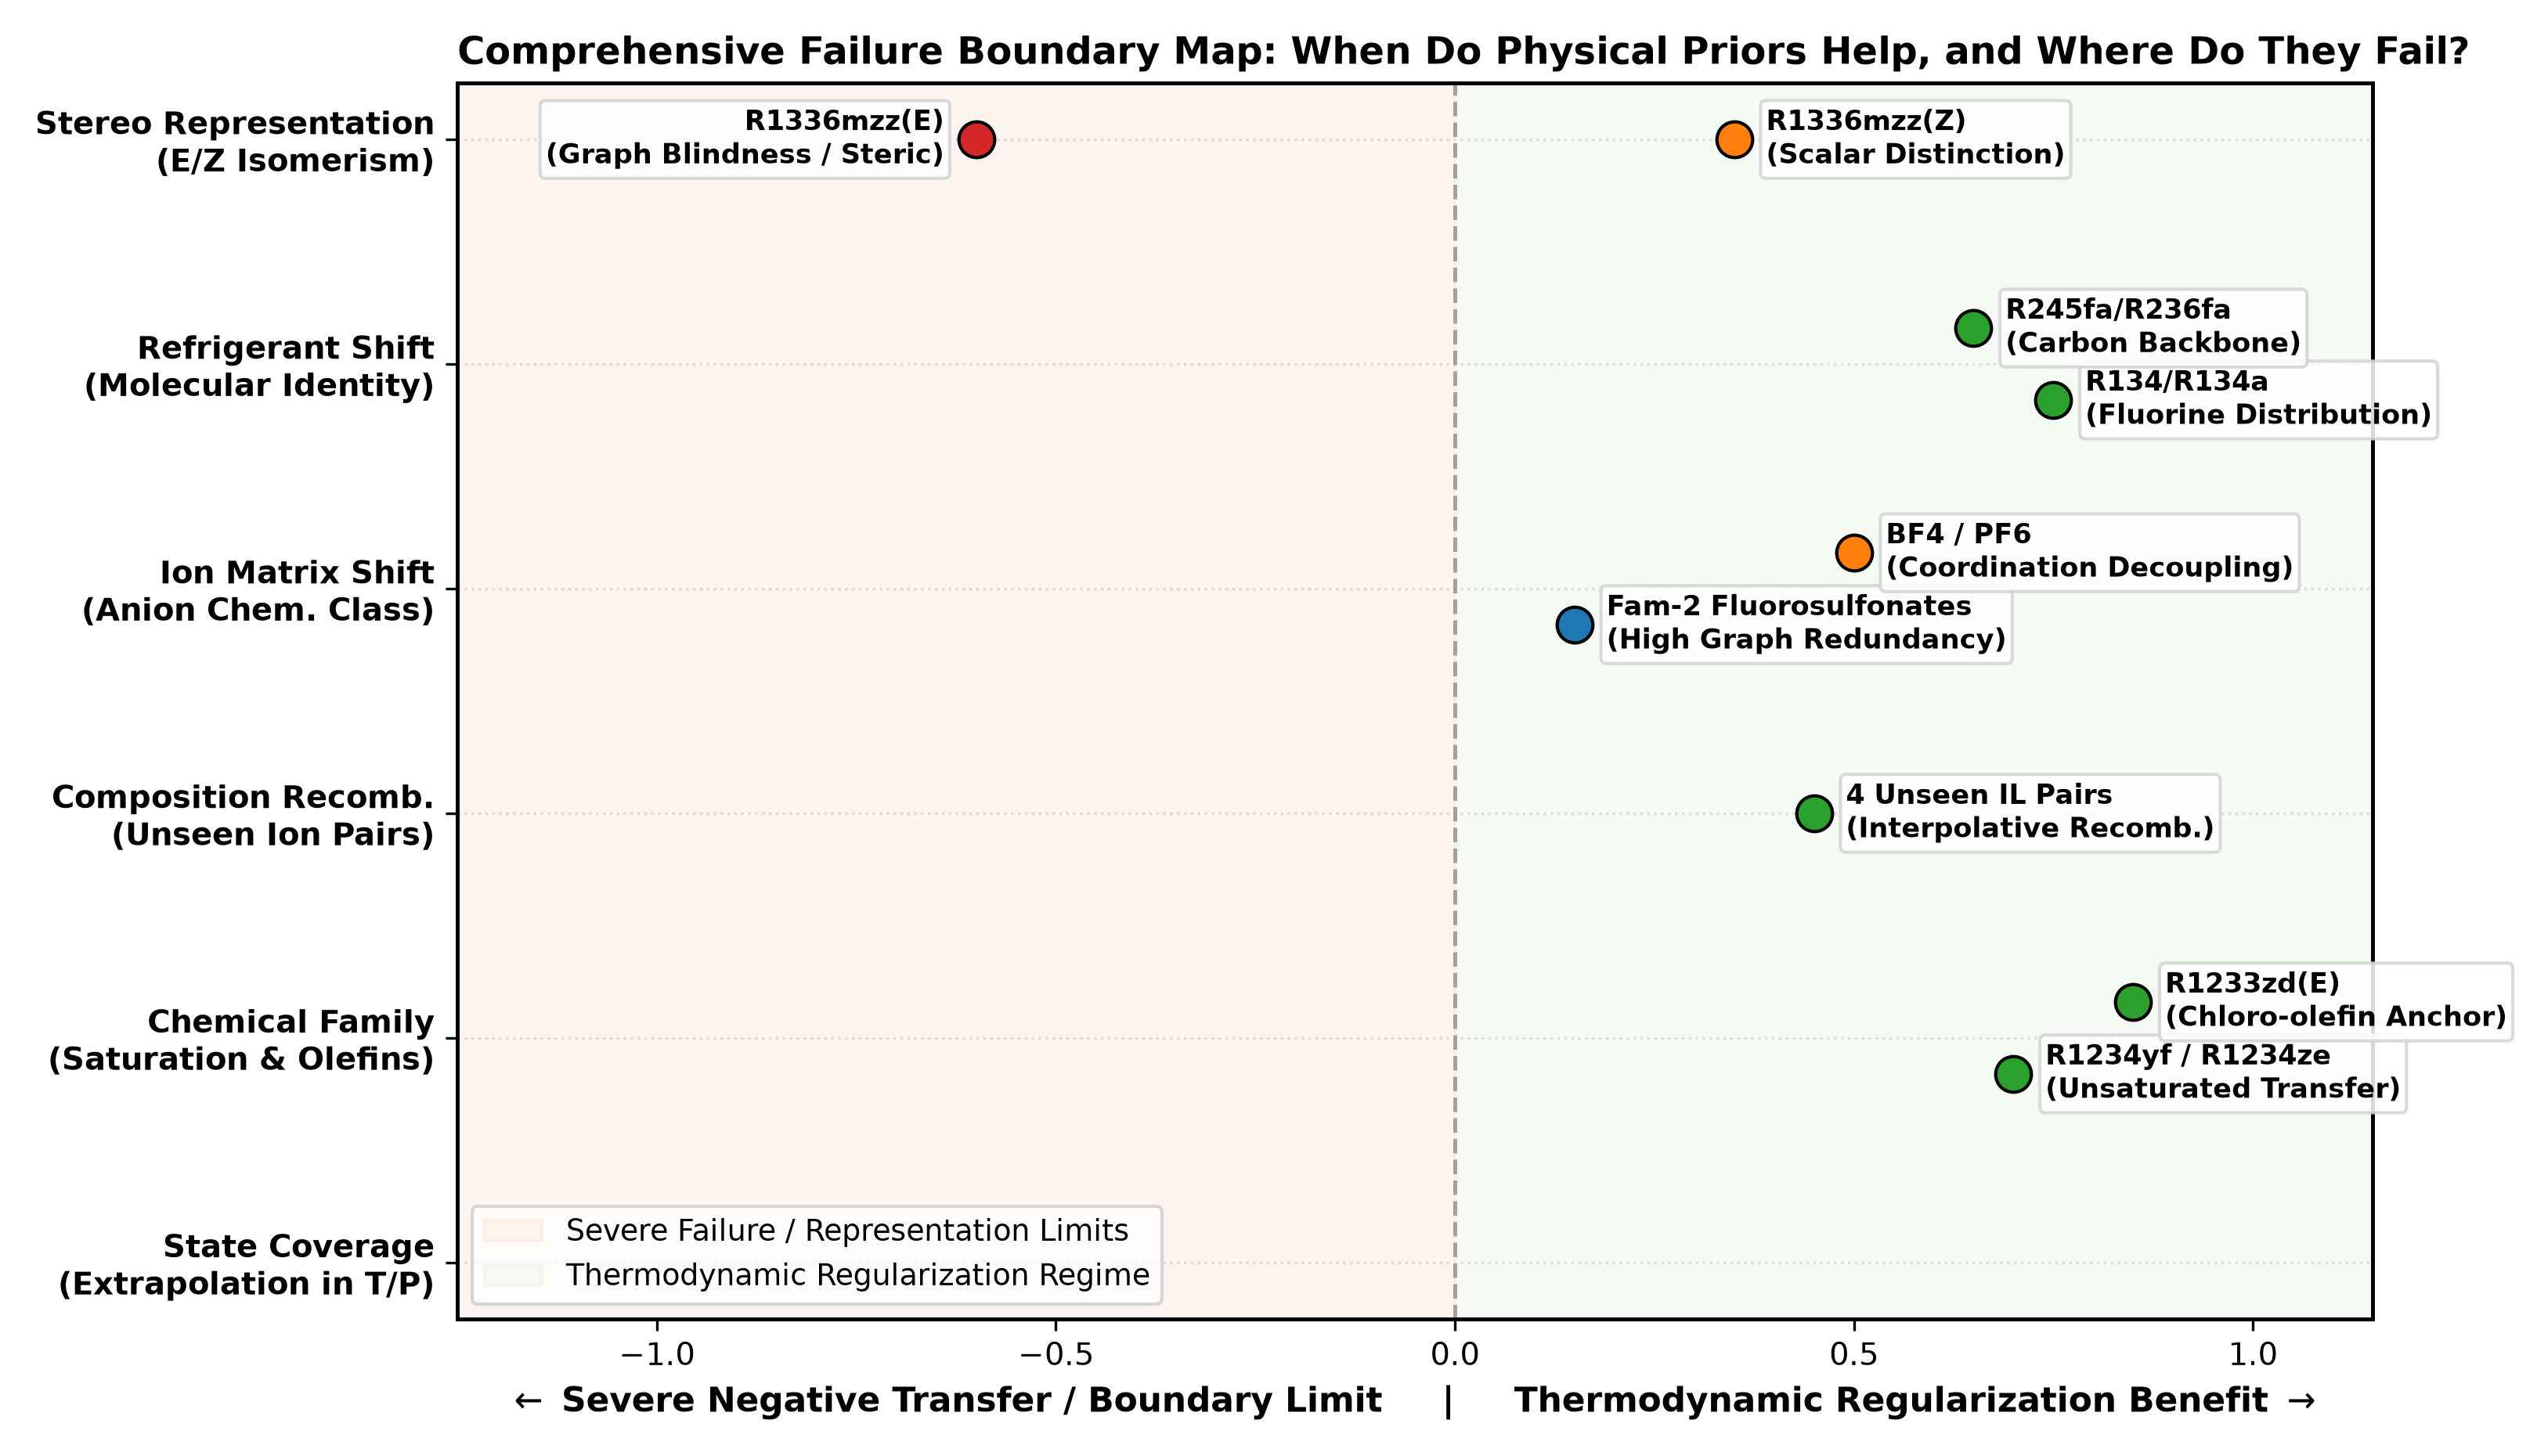
\includegraphics[width=0.88\linewidth]{figures/Figure5_failure_boundary_map.pdf}
\caption{\textbf{Comprehensive failure boundary and inductive bias taxonomy.} Two-dimensional taxonomy mapping chemical distribution shift dimensions against the effectiveness of thermodynamic regularization. While thermodynamic coordinates reliably regularize state extrapolation, olefin transfer, and structural isomers (green/orange), they fail to remediate stereochemical graph degeneracies such as R1336mzz(E) (red), demarcating the boundary between parameter regularizability and topological representation limits.}
\label{fig:figure5_boundary}
\end{figure}

\subsubsection{Error–Uncertainty Rank Association}
Across all evaluated OOD axes, the ensemble disagreement exhibits moderate to strong positive rank correlation with absolute prediction error ($\rho(\sigma, |e|)$ approximately $0.31\text{--}0.61$, Table~\ref{tab:uncertainty_risk}). The correlation is strongest on the anion-shift benchmarks (B2: $\rho = 0.6101$; B1: $\rho = 0.5062$) and the cross-family olefin benchmark (HFO: $\rho = 0.4926$). Notably, $M_{\mathrm{reduced}}$ substantially improves rank correlation relative to $M_0$ (e.g., in B1, $\rho$ increases from $0.2891$ to $0.5062$; in B2, from $0.4761$ to $0.6101$), indicating that physical priors stabilize ensemble consensus around true underlying thermodynamic trends.

\subsubsection{Selective Prediction Risk–Coverage Profiles}
In practical deployment, systems can utilize ensemble disagreement to trigger an abstention policy, referring high-uncertainty mixtures to experimental characterization or molecular dynamics simulations. As shown in Figure~\ref{fig:figure4_uq}b, sorting test samples by $\sigma_i$ and systematically rejecting the most uncertain predictions produces monotonically declining risk-coverage curves across all five axes:
\begin{itemize}
    \item In the B1 anion benchmark, abstaining on the top 50\% most uncertain samples reduces retained-set prediction error by \textbf{$52.5\%$} ($\text{MAE}: 0.0292 \to 0.0139$).
    \item In the B2 inorganic fluoride benchmark, 50\% selective coverage reduces retained-set prediction error by \textbf{$51.2\%$} ($\text{MAE}: 0.0472 \to 0.0230$).
    \item Across the HFO/HCFO, M1, and L2 benchmarks, selective prediction at 50\% coverage reduces retained-set MAE by $34.4\%$, $27.2\%$, and $25.8\%$, respectively.
\end{itemize}

We emphasize an important aggregation distinction for the M1 LORO axis: the reported ensemble MAE of $0.0613$ is macro-averaged across the 12 held-out refrigerants to weight each chemical species equally, whereas the risk–coverage evaluation pools all $N=1403$ test instances directly, yielding a full-coverage risk of $0.0720$ that progressively drops to $0.0524$ at 50\% coverage.

Crucially, however, ensemble disagreement is \textbf{not infallible}. On R1336mzz(E), because all five seeds inherited the identical degenerate 2D graph representation, the ensemble exhibits false confidence: R1336mzz(E) exhibited a relatively low ensemble disagreement ($\bar{\sigma} = 0.0213$) despite its large prediction error, indicating that ensemble disagreement may fail to detect representation-level blindness (Table~\ref{tab:unsat_species}). This underscores that while deep-ensemble disagreement can provide a useful ranking signal for some forms of parametric distribution shift, it cannot identify representational blindness caused by invariant graph topologies.
